In this section, we first describe the data sets used in our
experimental study. Follow that, we present the experiments to
evaluate our overall system and compare it with other systems using
existing large-scale resources. We also give a deeper understanding
about our system by performing several experimental analyses.

\subsection{Datasets}
\label{sec:dataset}

Our approach to identifying relational knowledge is evaluated by using
a dataset of 40 semantic classes of almost 11,000 instances, which was
used in \cite{citeulike:1587018}. This dataset was manually
constructed\footnote{Private communication with Marius Pasca, 2009.}
and was used to evaluate several information extraction tasks
\cite{citeulike:1587018,pacsca-vandurme:2008:ACLMain}.  Each semantic
class is an incomplete set of representative instances and has about
272 instances in average. The smallest class is {\em search engine}
with 25 instances, and the largest class is {\em actor} with 1500
instances. Table \ref{table:class-instance} shows a snippet of the
dataset. We have both types of closed word semantic
class (e.g. {\em chemical element}, {\em country}) and open word
semantic class (e.g. {\em basic food}, {\em hurricane}). Moreover,
there are classes with proper nouns (e.g. {\em actor} with {\em Mel
  Gibson}) and classes with common nouns
(e.g. {\em basic food} with {\em rice}, {\em milk}).

\begin{table}[!t]
\small
  \centering
  \begin{tabular}{|r|l|}
    \hline
    \multicolumn{2}{|c|}{A snapshot of the original dataset} \\
    \hline
    \textbf{Semantic class (Size)} & \textbf{Examples of Instances} \\
    \hline
    \hline
    basic food (155) & rice, milk, eggs, beans, fish \\
    \hline
    chemical element (118) & lead, copper, aluminum, calcium \\
    \hline
    city (589) & San Francisco, Dubai, Chicago \\
    \hline
    disease (209) & arthritis, hypertension, influenza \\
    \hline
    actor (1500) & Kate Hudson, Mel Gibson \\
    \hline
  \end{tabular}
  \caption{A snippet of 40 semantic classes with instances. 
    The class names in the original dataset ({\em basicfood}, 
    {\em chemicalelem}) were presented in a meaningful form
    as shown in the left column.}
  \label{table:class-instance}
\end{table}

In the original dataset, the semantic class names are not often
written in a meaningful form, such as {\em chemicalelem}, and {\em
  proglanguage}. These names are not valid
concepts. In our experiments, each semantic class name in the original
dataset is expanded to meaningful forms. For example, {\em
  terroristgroup} is expanded to {{\em terrorist group}, {\em
    terrorrist}, {\em torrorism}}. We use these expansions for all
systems in evaluation.

\begin{table}[!t]
  \small
  \centering
  \begin{tabular}{|r|l|l|}
    \hline
    \multicolumn{3}{|c|}{Concept pair examples} \\
    \hline
    Relation          & Concept $X$ & Concept $Y$    \\
    \hline
    \hline
    $X \leftarrow Y$        & actor             & Mel Gibson           \\
    & food              & rice                 \\
    % & wine              & Champagne            \\
    \hline                               
    $X \rightarrow Y$       & Makalu            & mountain             \\
    & Monopoly          & game                 \\
    % & krooni            & currency             \\
    \hline                               
    $X \leftrightarrow Y$   & Paris             & London               \\
    & copper            & oxygen                \\
    % & Nile              & Volga                 \\
    \hline                               
    $X \nleftrightarrow Y$ & Roja              & C++                  \\
    & egg               & Vega                  \\
    % & HotBot            & autism                \\
    \hline
  \end{tabular}
  \caption{Some examples in our data set.}
  \label{table:examples}
\end{table}


An example in our learning problem is a pair of two concepts ($X$,
$Y$) such as ({\em city}, {\em Dubai}), ({\em lead}, {\em
  aluminum}). Note that in this paper, we refer to both the name of
the semantic classes and their instances as concepts, such as {\em
  city} and {\em Dubai}. We pair the semantic classes and instances in
the original data set to create training and testing examples. The
examples cover all types of relational knowledge of interest: $X
\leftarrow Y$, $X \rightarrow Y$, $X \leftrightarrow Y$, and $X
\nleftrightarrow Y$. Specifically, examples are created with the
following guidelines.

\begin{itemize}
\item $X \leftarrow Y$ examples: For each semantic class, we pair the
  name of the class with its instances. These examples have the
  genearl form ({\em semantic class X}, {\em child of X}).
\item $X \rightarrow Y$ examples: These examples have the general form
  ({\em concept X}, {\em semantic class of X}).
\item $X \leftrightarrow Y$ examples: The general form of these
  examples is ({\em concept X}, {\em concept Y}), where $X$ and $Y$
  are two instances of a semantic class, and $X \ne Y$.
\item $X \nleftrightarrow Y$ examples: To make examples with two
  concepts having no relation, we pair either a semantic class name
  and an instance of another semantic class (and vice versa), or an
  instance in a semantic class and another instance in other classes.
\end{itemize}


We randomly create $20,000$ examples following the guidelines
above. Table \ref{table:examples} shows some examples created from the
original data set. We use $8,000$ examples for the training set, and
$12,000$ examples for the test set. We refer to the 12,000-example
test set as the {\em TestAll} test set. From the training set, we
discard examples with one or both concepts not in Wikipedia ({\em
  non-Wikipedia examples}). This results in a training set of $6,959$
examples.  It is important to note that, we do not discard {\em
  non-Wikipedia} examples in the {\em TestAll} test set. Table
\ref{tab:detail-dataset} shows the statistics of the training and
test data.

\begin{table}[!t]
  \small
  \begin{center}
    \begin{tabular}{|l||c|c|c|c|c|}
      \hline
      Data & $X \leftarrow Y$ & $X \rightarrow Y$  & $X \leftrightarrow Y$  & $X \nleftrightarrow Y$ & Total \\
      \hline
      \hline
      {\em Training}  & 1,739 & 1,754 & 1,664 & 1,802 & 6,959\\
      % {\em TestWiki} & 2,684 & 2,654 & 2,483 & 2,635 & 10,456 \\
      {\em TestAll} & 3,045 & 3,025 & 2,965 & 2,965 & 12,000 \\
      \hline
    \end{tabular}
    \caption{Details of the training and test sets with the number of
      examples in each relation class. The {\em Training} set contains
      only examples in Wikipedia. {\em TestAll} includes {\em
        non-Wikipedia} examples.}
    \label{tab:detail-dataset}
  \end{center}
\end{table}

To evaluate our system, we use a snapshot of Wikipedia from July,
2008. We first clean up articles in Wikipedia and remove articles that
are not of interest. The removed articles include articles without a
category, except the redirect pages, or articles with useless
categories such as {\em Protected redirects}. We also remove
administrative articles including {\em Wikipedia} pages, {\em
  Template} pages, {\em Image} pages, and {\em Portal} pages. We also
do not use articles without titles. After pre-processing, 5,503,763
articles remain. We index the articles using the Apache Lucene
Information Retrieval library\footnote{http://lucene.apache.org,
  version 2.3.2}. Lucene is a high-performance text search library
written in Java and widely used as an off-the-shelf IR system.

\subsection{Overall Results and Comparison}
\label{sec:exp-results}

To the best of our knowledge, no prior work directly targets the
problem of identifying the relational knowledge defined in this
paper. Most prior work which relates to our problem focuses on
building lexical taxonomy or knowledge ontology
\cite{Snow2006,wikitaxo07,suchanek2007WWW}. By searching the knowledge
base, one can find the answer for relationships between input
concepts. We compare our system with three other systems which are
built upon different existing resources.

\begin{table}[!t]
  \begin{center}
    \begin{tabular}{|c||c|c|c|c|}
      \hline
      \multicolumn{5}{|c|}{Overall results and comparison} \\
      \hline
      $K$  &  \textsc{Strube 07}  &  \textsc{Snow 06}  &  \textsc{Yago 07}  &  \textsc{Ours}            \\
      \hline
      1  &      23.83  &    40.24  &           64.43  &  \textbf{82.13}  \\
      2  &      23.84  &    42.63  &           63.94  &  \textbf{84.79}  \\
      3  &      23.88  &    40.96  &           62.02  &  \textbf{85.07}  \\
      4  &      24.32  &    40.65  &           60.57  &  \textbf{84.08}  \\
      \hline
    \end{tabular}
    \caption{Performance of our overall system compared to other
      systems. Performances are measured by accuracy. The {\em
        TestAll} test set with $12,000$ examples is used in this
      experiment. $K$ is the number of levels to climb up in the
      hierarchical structure of knowledge sources as described in the
      text.}
    \label{table:compare-others}
  \end{center}
\end{table}

\begin{table}[!t]
  \begin{center}
    \begin{tabular}{|c||c|c|c|c|}
      \hline
      \multicolumn{5}{|c|}{Comparison on special data sets} \\
      \hline
      Data set &  \textsc{Strube 07}  &  \textsc{Snow 06}  &  \textsc{Yago 07}  &  \textsc{Ours}   \\
      \hline
      {\em TestWiki}  &               24.59  &             44.34  &             70.29  &  \textbf{90.92}  \\
      {\em TestWn}    &               24.13  &             47.79  &             70.81  &  \textbf{90.76}  \\
      \hline
    \end{tabular}
    \caption{Comparison of systems' performance with different test
      sets derived from the {\em TestAll} test set. {\em TestWiki}
      contains $10,456$ examples in Wikipedia, and {\em TestWn}
      contains $8,625$ examples in the {\em extended WordNet}. The
      best performance of each system (by varying $K$) is reported.}
    \label{table:exp-diff-test}
  \end{center}
\end{table}

\begin{enumerate}

\item \textsc{Strube 07} uses a large scale taxonomy which was derived
  from Wikipedia \cite{wikitaxo07}, as the background knowledge. The
  taxonomy was created by applying several lexical matching and
  methods based on connectivity in the network to the category system
  in Wikipedia. As a result, the taxonomy contains a large amount of
  subsumption, i.e. {\em isa}, relations \cite{wikitaxo07}. Given an
  input with two concepts $X$ and $Y$, using the taxonomy, $X$ is an
  ancestor of $Y$ if one of the articles about $Y$ is subsumed by an
  article about $Y$, using {\em isa} links of articles, up to $K$
  levels in the taxonomy.  Similarly, for the case that $Y$ is an
  ancestor of $X$. If $X$ and $Y$ share a common ancestor within $K$
  levels in the taxonomy, they are considered siblings. We first apply
  our concept disambiguation algorithm on given concepts and then
  mount them onto the taxonomy to infer the relations. The taxonomy
  used in this experiment is in the latest version from March,
  2008\footnote{Private communication with Michael Strube and Simone
    Paolo Ponzetto, 2009.}.

\item \textsc{Snow 06} uses the {\em extended WordNet}
  \cite{ilprints665,Snow2006} as background knowledge. To build the
  {\em extended WordNet}, the authors first identified
  lexico-syntactic patterns indicative of hypernymy from
  corpora and use them to extract candidate noun pairs
  that may hold the hypernym relation. A trained classifier is applied
  on these noun pairs to recognize the pairs holding hypernym
  relation. Starting from WordNet-2.1 \cite{Fellbaum98}, the latest
  version of the extended WordNet has augmented 400,000 synsets. Words
  that are added into the extended WordNet can be common nouns or
  proper nouns. The extended WordNet can serve as effective background
  knowledge for identifying the relational knowledge of interest by
  looking for the input concepts in the extended WordNet tree in all
  possible senses of the concepts and then inferring their
  relationship. We also vary the value of $K$ as the number of levels
  to go up on the WordNet tree from input concepts to find their
  common subsumptions.

\item \textsc{Yago 07} uses YAGO ontology \cite{suchanek2007WWW} as
  the main source of background knowledge. Because YAGO ontology is a
  combination of Wikipedia and WordNet (see our brief description in
  Sec. \ref{sec:rel-con-ext}), this system is expected to be powerful
  in recognizing concept relationships. To access a concept's
  ancestors and siblings, we combine \textsc{Pattern 1} in
  Fig. \ref{alg:yago-query} and the \textsc{subClassOf} relation in
  YAGO model to go up on the ontology. The \textsc{subClassOf}
  relation can be cascaded $K$ times to climb up in the ontology.

\end{enumerate}

Our system, \textsc{Ours}, is described in
Fig. \ref{fig:rel-know-iden-alg}. All systems are evaluated on the
{\em TestAll} test set with $K$ from 1 to 4. Table
\ref{table:compare-others} shows the comparison of the systems in
details. It is shown that our system significantly outperforms other
systems implemented using existing sophisticated resources. Our
system also uses Wikipedia as its main background
knowledge. However, ours is superior to other systems because it
employs advance machine learning techniques along with a powerful and
effective constraint-based inference model.

Because the systems in the previous experiments do not use the same
source of background knowledge, we, furthermore, perform experiments
in which these systems are compared with different data sets covered
in different knowledge sources. This experiment provides a fair
comparison for systems that use different resources as their
background knowledge. New data sets are derived from the {\em TestAll}
test set. The first derived data set is {\em TestWiki} which contains
only {\em Wikipedia concepts}. By removing all examples with {\em
  non-Wikipedia concept}, there are $10,456$ examples remained in {\em
  TestWiki}. The second derived data set is {\em TestWn}, which
contains only concepts in the {\em extended WordNet}
\cite{ilprints665,Snow2006}.  {\em TestWn} has $8,625$ examples after
dropping $3,375$ examples with concepts not in the {\em extended
  WordNet} from {\em TestAll}.  The results of this experiment are
shown in Tab. \ref{table:exp-diff-test}.  We only report the best
results achieved by the systems on different test sets. Our system
still significantly outperforms other systems when compared on
specific data sets.


\subsection{Experimental Analysis}

\begin{table*}[!t]
  \begin{center}
    \begin{tabular}{|l||c|c|c|}
      \hline
      \multicolumn{4}{|c|}{Contributions of the components in our system} \\
      \hline
      &         Results on $10,456$  &  Results on $1,544$              &         Overall results  \\
      System &  {\em Wikipedia examples}  &  {\em non-Wikipedia examples}  &  on $12,000$ examples  \\
      \hline
      \hline
      Baseline        &                       88.79  &                      31.22       &                   81.38  \\
      \hline
      w/o Inference   &                       88.79  &                      44.88       &                   83.14  \\
      \hline
      with Inference  &                       \textbf{90.92}  &                      \textbf{45.40}       &                   \textbf{85.07}  \\
      \hline
    \end{tabular}
    \caption{Contributions of the components in our system evaluated
      on three types of data. The first column shows results only on
      examples with concepts that appear in Wikipedia. The second
      column shows results on examples having concepts that do not
      appear in Wikipedia, and thus exhibits the power of our method
      to extend outside Wikipedia. The third column shows results on
      the overall data set, that consists of around 13\% of the
      concepts pairs that are outside Wikipedia. The {\em Baseline}
      system is our local relation classifier that uses neither the
      approach of finding replacements for {\em non-Wikipedia
        concepts} nor the inference model. The baseline on {\em
        non-Wikipedia examples} is computed by assuming sibling
      relation all the time. By adding the component of finding
      replacements for {\em non-Wikipedia concepts}, we have the {\em
        w/o Inference} system.}
    \label{tab:w-wo-infer}
  \end{center}
\end{table*}

In this section, we give several experimental analyses on our system.
These analyses provide a deeper understanding of different aspects on
our system.

\subsubsection{Contributions of the Components in our System}

In this experiment, we show the contribution of the components in our
overall algorithm (see Fig. \ref{fig:rel-know-iden-alg}). We use
different data sets in this experiments to study the variation in
behavior of our system. The first data set is the {\em TestWiki} in
the previous experiment. This test set contains $10,456$ examples with
{\em Wikipedia concepts}. These are the remained examples after
dropping {\em non-Wikipedia concepts} from $12,000$ examples in the
{\em TestAll} test set. The second test set contain only $1,544$
concept pairs with at least one {\em non-Wikipedia} concept in
each. In other words, the second test set is the complement of the
{\em TestWiki} test set with respect to the {\em TestAll} test
set. The third test set is the {\em TestAll} test set. The results are
shown in Tab. \ref{tab:w-wo-infer}.

In Tab. \ref{tab:w-wo-infer}, the {\em Baseline} system is our local
relation classifier that uses neither the component finding
replacements for {\em non-Wikipedia concept} nor the constraint-based
inference model. The baseline on {\em non-Wikipedia examples} is
computed by assuming sibling relation all the time. In the {\em w/o
  Inference} row, we evaluate our system with the contribution of the
component finding replacements for {\em non-Wikipedia concepts}, but
inference model. The result on $10,456$ {\em Wikipedia examples}
remains the same because, all of concepts in these examples are in
Wikipedia, the system does not need to find replacement concepts. The
significant improvement in the results on $1,544$ {\em non-Wikipedia
  examples} shows the effectiveness of our approach in finding
replacements for {\em non-Wikipedia concepts}. Overall, we obtain
almost $2\%$ of improvement in accuracy after adding the finding
replacement component. The third experiment is carry out by evaluating
our overall algorithm in Fig. \ref{fig:rel-know-iden-alg} on all test
sets. The inference process significantly improve the results of our
system on $10,456$ {\em Wikipedia examples}. It also gains
improvements on the {\em non-Wikipedia examples} so that in overall,
by adding the constraint-based inference component, the system improves
$\sim 2\%$ in accuracy. Overall, our system achieves
significant improvement reaching to $85.07\%$ accuracy in overall by
adding in all components, compared to $81.38\%$ accuracy gained by the
{\em Baseline} system.



\begin{table*}[!t]
  \begin{center}
    \begin{tabular}{|c|c|c|c|c|c|c|c|}
      \hline
      No.  &  $X$             &  $Y$          &  True    &  LocalClassifier       &  \multicolumn{2}{|c|}{Replacement Needed?}  &  withInference \\ \cline{6-7}
      &                  &               &  Label   &  Prediction                   &  $X$                  &  $Y$                     &  Prediction           \\
      \hline
      \hline
      1&city                    &lisbon                   &$\mathbf{X \leftarrow Y}$      &$\mathbf{X \leftarrow Y}$      &(no)        &(no)         &$\mathbf{X \leftarrow Y}$  \\
      2&{\em bartlomiej strobel}&painter                  &$\mathbf{X \rightarrow Y}$     &$\mathbf{X \rightarrow Y}$     &drew struzan&(no)         &$\mathbf{X \rightarrow Y}$ \\
      3&taiwan                  &singapore                &$\mathbf{X \leftrightarrow Y}$ &$X \leftarrow Y$               &(no)        &(no)         &$\mathbf{X \leftrightarrow Y}$ \\
      4&jean ingres             &{\em harald slott-moller}&$\mathbf{X \leftrightarrow Y}$ &$X \nleftrightarrow Y$         &(no)        &george inness&$\mathbf{X \leftrightarrow Y}$ \\
      5&{\em southern herald}   &newspaper                &$\mathbf{X \rightarrow Y}$     &$X \leftrightarrow Y$          &liberty     &(no)         &$\mathbf{X \rightarrow Y}$  \\
      6&somalia                 &hurricane                &$\mathbf{X \nleftrightarrow Y}$&$\mathbf{X \nleftrightarrow Y}$&(no)        &(no)         &$X \leftrightarrow Y$  \\
      \hline
    \end{tabular}
    \caption{Relationship prediction examples from {\em TestAll} test
      set. Concepts in {\em italic font} are not in Wikipedia, and
      they are replaced by other {\em Wikipedia concepts} as shown.}
    \label{table:pre-examples}
  \end{center}
\end{table*}

\subsubsection{Contribution of Related Concepts in Inference}
\label{sec:contr-relat-conc}

\begin{figure}[t]
\centering
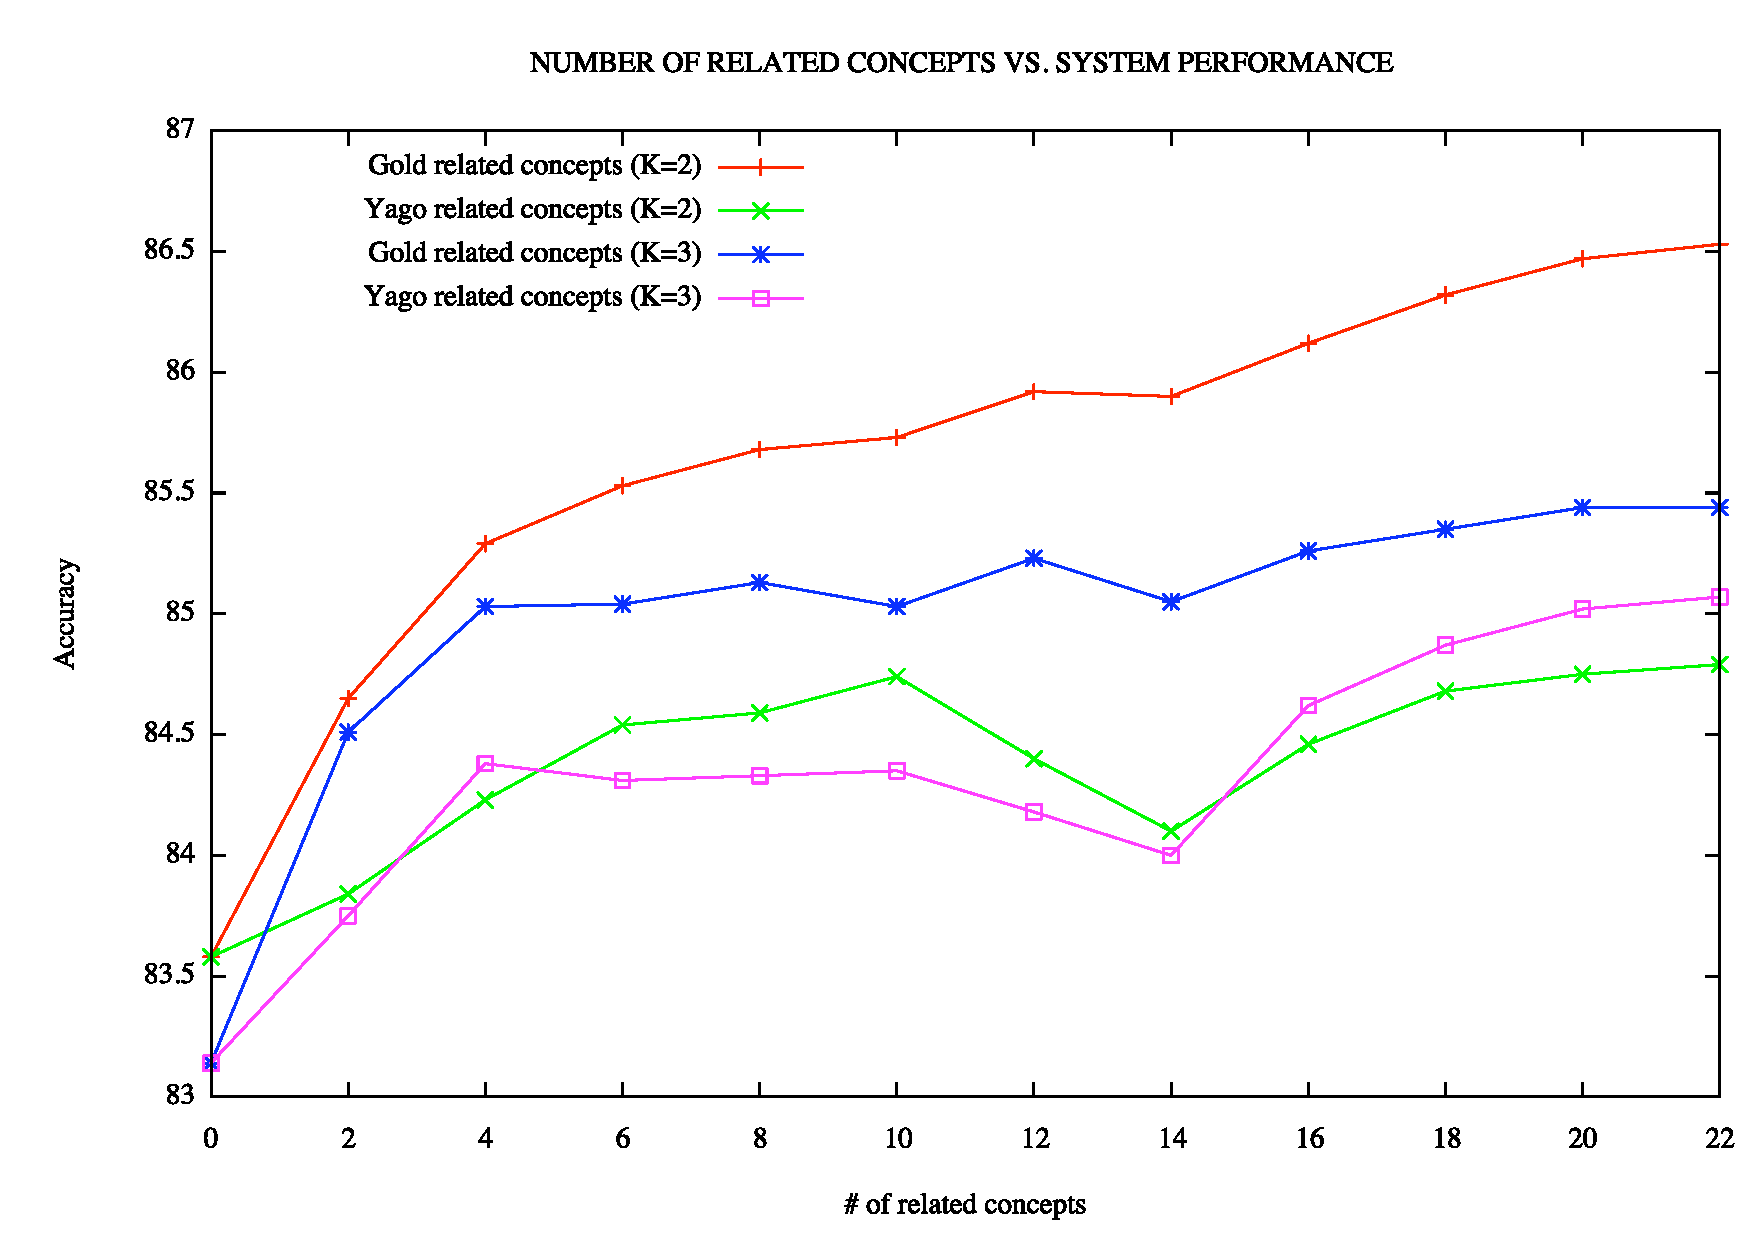
\includegraphics[totalheight=0.25\textheight]{relatedconcepts4}
\caption{Relation between our system performance and the number of
  related concepts used in the constraint-based inference model.}
\label{fig:related-concepts}
\end{figure}

In our inference process, we used related concepts added to form
relational constraints in concept networks. The relational constraints
will then enforce concept networks to eliminate violated ones and pick
the best concept network available. From our inference model, we make
two following claims: (1) The more relevant to the input concepts the
related concepts are, the better performance the system gets, and (2)
the more related concepts added to the inference process, the better
performance the system gets.

To prove the first claim, we use the original data of forty semantic
classes (see Sec. \ref{sec:dataset}) to provide {\em gold related
  concepts} to the inference process as discussed in
Sec. \ref{sec:rel-con-ext}. Our experiment shows that by using this
approach, the performance of our best system reaches to $86.52\%$ in
accuracy on the {\em TestAll} test set, compared to $85.07\%$ accuracy
obtained when using another knowledge source to provide related
concepts. For the second claim, we evaluate our system with several
numbers of related concepts added to the inference process. In this
experiment, we use both the {\em gold related concepts} provided by
the original dataset and the {\em YAGO related concepts} extracted
from YAGO ontology (see Sec. \ref{sec:rel-con-ext}) for the inference
process.

Fig. \ref{fig:related-concepts} shows the improvement in the
performance of our system with respect to the quality of the related
concepts used and also the number of related concepts. This experiment
is done on the {\em TestAll} test set. It is shown clearly that the
related concepts from gold data outperform the related concepts
extract from the other source. Due to the quality of the related
concepts extracted from YAGO ontology, sometimes, adding more concepts
hurts the performance. We use $K=2$ and $K=3$ in this
experiment\footnote{$K$ is the number of levels to go up in the
  Wikipedia category system to extract features for input concept
  pairs.}. The related concepts include the ancestors, siblings, and
children of an input concept. For simplicity, in this experiment we
only report the total number of related concepts extracted for two
input concepts of an example.

\subsubsection{System's Output Examples}

Table \ref{table:pre-examples} shows some output examples of our
overall system in Fig. \ref{fig:rel-know-iden-alg} (see column {\em
  withInference}). We also present the predictions made by the system
without inference component ({\em LocalClassifier}). Concepts which
are not in Wikipedia will be replaced by {\em Wikipedia concepts}
({\em Replacement Needed?}). Example \#1 and \#2 show two concept pairs
correctly classified by both {\em LocalClassifier} and {\em with
  Inference}. Especially, in \#2, that concept {\em bartlomiej
  strobel} is replaced with {\em drew struzan} helps the systems make
correct predictions. In examples \#3, {\em LocalClassifier} make
incorrect predictions, but {\em withInference} remedies this. Example
\#4 and \#5 show two cases where two {\em non-Wikipedia concepts} are
correctly replaces with two corresponding {\em Wikipedia concepts},
but {\em LocalClassifier} still makes incorrect prediction. However,
{\em withInference}, with its power of internal reasoning using
relational constraints, proves to be successful. Example \#6 is an
example where {\em LocalClassifier} makes correct prediction, but {\em
  withInference} does not. This is probably because of bad related
concepts extracted for the two input concepts.

%%% Local Variables: 
%%% mode: latex
%%% TeX-master: "jupiter"
%%% End: 
